\chapter{\textbf{Desarrollo}}

\thispagestyle{empty}

En el presente capítulo se detalla la planificación siguiendo la metodología Turpial Agile Unified Process (TAUP). Adicionalmente, se describe la evolución del proyecto y sus dificultades, así como las actividades realizadas que llevaron a cumplir los objetivos planteados y logros adicionales.

\section{Fase de concepción}

En esta sección se detallan las funcionalidades de los módulos Principal (\textit{Core}) y Estadísticas de la librería Auditorías Turpial según los requerimientos del cliente; y se muestra el diseño de la solución y  planteamiento de la arquitectura. También, se elaboran los documentos según TAUP y se definen las tecnologías necesarias para el desarrollo del proyecto. Este proceso abarcó las primeras cuatro semanas de la pasantía.

\subsection{Análisis de requerimientos}

Antes de tomar alguna decisión de implementación, fue necesario establecer cuál es la tecnología a la que va dirigida el producto final y cuáles son las funcionalidades mínimas que debe poseer. En primer lugar, se decidió que se desarrollaría una librería en Django, para Django, ya que la empresa suele utilizar este herramienta en sus aplicaciones; y utilizaría una base de datos relacional, en particular PostgreSQL, MySQL o SQLite porque se integran fácilmente al \textit{framework} . \\

En segundo lugar, se determinaron las Historias de Usuario (HU). La librería consta de tres módulos: \textit{Core}, Estadísticas y Reportes. El líder del proyecto se encargó de las HU correspondientes al módulo Principal y el pasante realizó el levantamiento de requerimientos del módulo de Estadísticas (ver apéndice C) según las necesidades del cliente. Adicionalmente, elaboró los documentos correspondientes, Documento de Requerimientos y \textit{Release Plan} siguiendo las plantillas de la empresa. \\

En este caso en particular, el rol del cliente lo interpretó la empresa misma, puesto que el producto será ofrecido como un servicio a clientes externos. El rol de \textit{product owner} lo desempeñó el tutor industrial para gestionar el desarrollo de la pasantía. \\

Para escribir las HU, es indispensable contar con el actor que ejecuta alguna acción específica, por lo que se distinguieron dos tipos de usuarios:

\begin{itemize}
    \item El programador, quien descargará la librería y la incluirá en la aplicación de Django que está desarrollando.
    \item Los “usuarios” finales, quienes utilizarán la aplicación en donde se instale la librería y la interfaz gráfica provista.
\end{itemize}

En líneas generales, el módulo \textit{Core} debe contar con las siguientes características:

\begin{itemize}
    \item Seleccionar cuál modelo (tabla) es auditable.
    \item Registrar el autor, acción, fecha, estado anterior y estado actual de una instancia particular en formato JSON. Las acciones auditables son: Crear, Actualizar y Eliminar.
    \item Listar todas las operaciones, filtrarlas y ordenarlas.
    \item Restringir el acceso del personal no autorizado a los listados.
    \item Proveer etiquetas personalizadas para las plantillas de los listados que faciliten la inclusión de los mismos.
\end{itemize}

El módulo de Estadísticas debe proveer el cálculo del total de auditorías, cantidad de modelos auditables, porcentaje de cobertura, porcentaje de crecimiento de los datos, promedio por día, mínimo y máximo. Dichos resultados pueden estar filtrados por un rango de tiempo, por acción, por autor y por modelo. Asimismo, debe contar con facilidades para incluir los gráficos que representen los cálculos mencionados anteriormente. \\

El módulo de Reportes ofrece la posibilidad de generar archivos sobre los listados en diversos formatos (CSV y PDF) y personalizar su apariencia con opciones como modificar los márgenes, espacios, incluir el nombre y logo del sistema, entre otros. Adicionalmente, la librería debe ser mantenible, eficiente, simple, confiable, escalable y fácil de integrar y configurar.\\

Por otro lado, es indispensable que se instalen automáticamente las dependencias de la librería en el sistema que la utilice para facilitar su uso y evitar errores. También, se requiere que la librería se actualice mediante el uso de una herramienta de integración contínua. \\

En esta pasantía se abarcarán las funcionalidades correspondientes a la selección del modelo auditable, registro de traza de auditoría y listados (sin filtros ni ordenamiento) del módulo \textit{Core} y completamente el módulo de Estadísticas con sus respectivas pruebas automatizadas. También se incluye la instalación y configuración del sistema de integración contínua. El módulo de Reportes está fuera del alcance.

\subsection{Adaptación de la metodología a la pasantía}

En el capítulo anterior se explicó la metodología TAUP, sin embargo, dependiendo del proyecto que se desea desarrollar, se pueden realizar algunas modificaciones que mejoren la dinámica y la velocidad del equipo o porque el cliente así lo requiera.

Se ideó un código compuesto por una letra y un número que facilita referenciar las HU. La letra representa el módulo a la que pertenece, \textit{Core} o Estadísticas, y el número denota el orden en que fue concebida. Adicionalmente, se utilizó una modificación  para las escalas de prioridad y riesgo, que está conformada por tres valores: Alta, Media y Baja. Para más información sobre las HU desarrolladas, leer el Apéndice C.

Por otro lado, se agregaron nuevos criterios a la \textit{Definition of Ready}, con lo que se tiene lo siguiente:

\begin{itemize}
    \item Debe ubicarse dentro de uno de los módulos del proyecto.
    \item Debe de tener asignado una prioridad por el cliente.
    \item Debe de tener asignado un riesgo por el equipo de desarrollo.
    \item Debe de tener asignado su respectivo puntaje.
    \item (Opcional pero deseado) Debe de tener una breve descripción, aclaratoria o criterio adicional según sea el caso.
\end{itemize}


Asimismo, se amplió la \textit{Definition of Done} para agregar las pruebas automatizadas de cada HU. Posee los siguientes estatutos:

\begin{itemize}
    \item Debe realizarse la codificación respectiva
    \item El código generado debe estar debidamente documentado para facilidad de programador
    \item Debe de realizarse la documentación respectiva (de ser necesaria) de todos los aspectos de configuración asociados al desarrollo y buen funcionamiento de la historia de usuario.
    \item Deben realizarse pruebas automatizadas a la codificación generada.
    \item Debe presentarse la nueva funcionalidad al cliente.
    \item Debe estar disponible en el repositorio.
\end{itemize}

\subsection{Arquitectura propuesta del sistema}

El planteamiento inicial (Figura 6.1) consistía en desarrollar cada módulo de la librería en una aplicación de Django distinta, las cuales se instalarían por separado en el sistema, el cual será referido como “Host” para simplificar la notación. Los módulos de Estadística y Reportes serían ofrecidos como microservicios dependientes del módulo principal pero independientes entre ellos, de manera que si alguno falla, el otro no sea afectado.\\

\begin{figure}
\centering
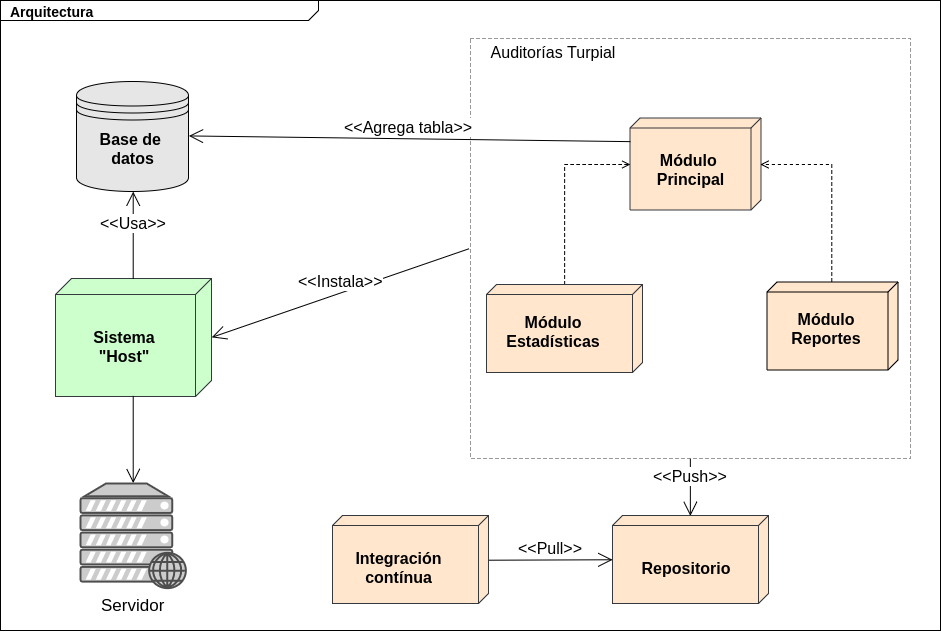
\includegraphics[width=\textwidth]{Diagrama_Arquitectura.png}
\caption{Arquitectura de la librería Auditorías Turpial}
\label{fig:figure6.1}
\end{figure}

Se decidió que el módulo Principal agregaría una nueva tabla en la base de datos ya existente del “Host” en la que mantendrá la información acerca de las auditorías y los otros módulos podrían leerla para procesarla y mostrarla como sea  pertinente.\\

No obstante, la arquitectura mostrada en la figura 6.1 sufrió modificaciones durante el desarrollo  el proyecto para simplificarla. En lugar de crear tres aplicaciones, una para cada módulo, se separó Auditorías Turpial en dos: \textit{backend} y \textit{frontend}. En la sección que explica la fase de construcción se ofrecerán mayores detalles de estos cambios y sus razones.

\begin{figure}
\centering
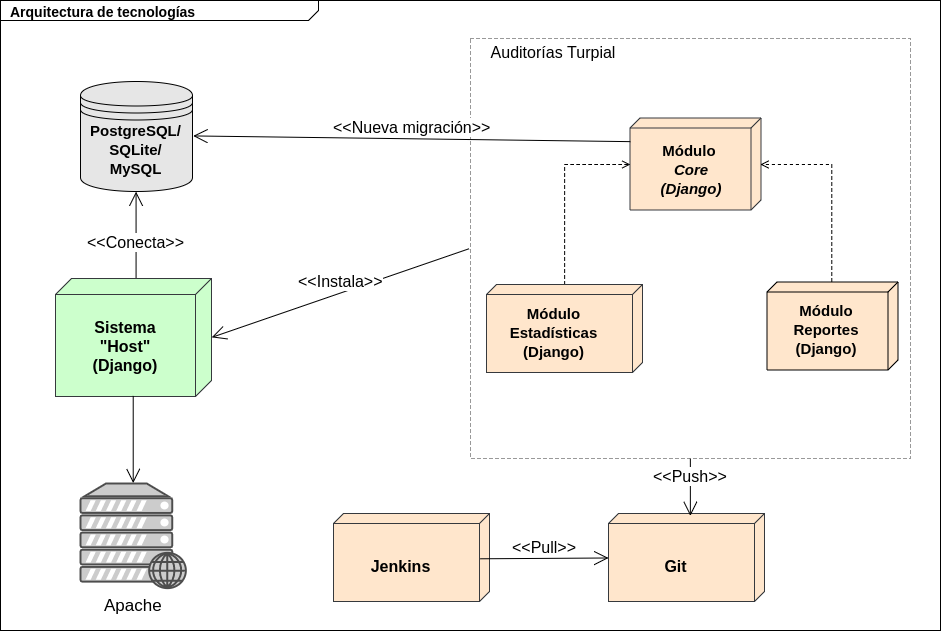
\includegraphics[width=\textwidth]{Diagrama_Tecnologias.png}
\caption{Arquitectura de tecnologías a utilizar}
\label{fig:figure6.2}
\end{figure}

En la figura 6.2 se muestran las tecnologías a utilizar en el proyecto. Como se mencionó anteriormente, se utilizará Django para el desarrollo. Como herramienta de control de versiones se utilizará Git y para automatizar la integración contínua se usará Jenkins. El sistema “Host” será un proyecto de la empresa que utilizará como servidor Web, Apache y una base de datos relacional.

\section{Diseño del módulo principal}

Uno de los problemas más significativos que la empresa encuentra en otras extensiones de Django disponibles, es el hecho de que el registro de auditoría se guarda a nivel de la vista y es responsabilidad del programador colocar el código para esta funcionalidad. Esto da cabida a que se olvide colocar en alguna de las vistas correspondientes a algún modelo, por lo que podría no guardarse todos los tipos de operaciones. \\

La librería Auditorías Turpial pretende evitar este problema guardando el registro de auditoría cada vez que ocurre alguna operación sobre el modelo a través del uso de las señales (\textit{signals}) que ofrece el \textit{framework} . Éstas señales, necesariamente deben distinguir entre un modelo auditable y uno que no lo es. Para esto, se contempló el uso de un \textit{mixin} que pueda ser heredado por cualquier modelo y así proveer todas las funcionalidades mencionadas. \\

Por otro lado, se desea incluir en las auditorías el usuario que realizó la acción. La solución mencionada anteriormente no es suficiente para lograr esto, puesto que a nivel de modelos no se posee información sobre el \textit{request} y no se puede saber qué usuario está en sesión. Por esta razón, se planteó agregar otro \textit{mixin} a nivel de vistas que completara la información antes de guardarla en la base de datos. Sería responsabilidad del programador heredarlo en todas las vistas cuyos modelos mantienen un historial de transacciones.
 \\

Django posee mecanismos para traducir los modelos a otro formato con una estructura bien definida, más conocidos como \textit{serializers} (serializadores), y viceversa. En particular, posee maneras de convertirlos a JSON, por lo que se decidió utilizar dicha funcionalidad para cumplir con el requisito de mostrar los cambios en los valores de los campos del modelo auditable en este formato.\\

En cuanto a los listados, se acordó utilizar Datatables para mostrarlos como una tabla que se pueda ordenar y filtrar fácilmente. Este \textit{plugin} puede manejar aproximadamente 10000 filas en sus tablas procesándolas del lado del cliente, sin embargo, las auditorías serán potencialmente millones de registros, es por esta razón se debe realizar el procesamiento del lado del servidor. \\

Para la autenticación se consideró utilizar un tabla de usuarios propia con su respectiva permisología, con la intención de que no interfiriera con la del sistema “Host”, sin embargo, esto no fue posible. Se ahondará en la explicación de esta decisión en la fase de desarrollo del presente capítulo.

\subsection{Diseño del módulo de estadísticas}

Uno de los requisitos mínimos con el que debe contar el módulo de Estadísticas es exponer un conjunto de gráficas que permitan visualizar e interpretar fácilmente los resultados de los cálculos de las auditorías. Para esto, se investigaron dos librerías de JavaScript: Amcharts y Charts.js. En la siguiente tabla se muestran las características principales:

%%%%% tabla%%%%

Como los desarrolladores de Turpial Development son los principales usuarios de este proyecto, el pasante investigó si existía alguna librería que utilicen usualmente. En la empresa han utilizado varias, incluyendo las dos presentadas anteriormente, por lo que no tienen una preferencia en este sentido. \\

Debido a que la cantidad de registros de auditorías pueden crecer rápidamente, es necesario escoger una librería de gráficos que maneje adecuadamente grandes volúmenes de datos, por lo que se decidió utilizar Amcharts. Otra característica que inclina la balanza a favor de esta solución, es el hecho de que posee un \textit{plugin} que permite exportar datos a un archivo CSV o PDF, una funcionalidad que se compenetra bien con el módulo de Reportes. \\

Aunque Charts.js posee una extensión de Django para facilitar la creación de los gráficos a través de las vistas, este proyecto requiere una lógica muy específica para entregar el conjunto de datos que se utilizará para renderizarlos. Por esta razón, es mejor tener total control sobre su implementación. \\

Los cálculos estadísticos serán entregados a la plantilla a través de una vista que incluirá el formulario de los filtros y la manipulación de los datos para crear los gráficos pertinentes y según los requiera la librería escogida.

\subsection{Propuesta para la integración continua}

Dado que en la empresa no existe precedente sobre el uso de una herramienta automatizada para integrar el código de manera continua, se le otorgó al pasante la libertad de escoger entre dos herramientas sugeridas por el líder del proyecto: Jenkins o Fabric. Para decidir cuál herramienta se adecuaba más al proyecto y a las necesidades de la empresa, fue indispensable que el pasante investigara las opciones en profundidad, sus fortalezas, limitaciones y recomendaciones de la comunidad. A continuación se muestra una comparación entre ellas:

%%% tabla%%%%

Considerando las características que posee cada herramienta, se decidió utilizar Jenkins puesto que se pueden ejecutar \textit{scripts} de manera programada, generar reportes, observar el estado del despliegue de varios proyectos e incluso integrarlo con Gitlab, un servicio Web de control de versiones y desarrollo de \textit{software} colaborativo basado en Git que es utilizado por la empresa. \\

Si bien Fabric es más simple, no es realmente un servidor para integración continua, se asemeja más a \textit{scripts} que permiten automatizar tareas y se requiere de una herramienta suficientemente general que pueda ser usado tanto en la pasantía como en otros proyectos de la empresa.

\subsection{Plan de pruebas}

Para verificar que cada funcionalidad posea el comportamiento esperado, se realizaron pruebas de manera automatizada utilizando Pytest. Más específicamente, se llevaron a cabo pruebas unitarias, de regresión y de integración.

Adicionalmente, se convino que uno de los criterios de aceptación de las HU era validar el producto con el cliente para asegurar el cumplimiento de las reglas de negocio y que el producto desarrollado cumple los estándares. A esto se le conoce como pruebas de aceptación y fueron realizadas en cada cierre de \textit{Sprint}.

Como el proyecto en cuestión es una librería, no puede funcionar por sí sola, sino que necesita instalarse en otro. Para esto, se creó una aplicación sencilla en Django y se instaló la librería en él. En cada \textit{Sprint}, se constató que el programador pueda usar cada funcionalidad desarrollada  sin ningún inconveniente. Este mismo proyecto, se utilizó para mostrar los avances al cliente.\\

En la fase de transición, se planificó que se realizaran pruebas en una aplicación desarrollada para uso interno de la empresa, llamado Turpial Team, cuyo propósito es gestionar empleados y permitir que conozcan a su equipo de trabajo. No obstante, debido a que aún se encuentra en desarrollo no está disponible actualmente. Se optó por utilizar otro proyecto de uso interno de Turpial Development, llamado Turpial Calendar. Esta aplicación sirve para planificar eventos de la empresa y enviar notificaciones. Esta decisión no afecta de ninguna manera la pasantía ya que la librería debe poder ser instalada en cualquier proyecto con las características mencionadas en la sección de requerimientos.

\subsection{Planificación del desarrollo del proyecto}

Luego de finalizar el proceso de investigación, aclarar los requerimientos y determinar las HU, se procedió a planificar la fase de construcción del proyecto. Para ello, se tomó en cuenta la prioridad, precedencia y puntaje de cada HU para determinar el orden. Se decidió iniciar con las HU relacionadas con el \textit{Core} y la instalación de la librería.\\

Se planificaron ocho \textit{Sprints} con una duración de dos semanas laborales (diez días) cada uno. Estos \textit{Sprints} abarcan la fase de construcción del módulo \textit{Core} y Estadísticas de Auditorías Turpial, así como la fase de transición.

\section{Fase de construcción}

Una vez culminada la fase de concepción, se procedió con la instalación del ambiente de desarrollo e implementación de los módulos que abarca la pasantía. También, se incluyen las pruebas pertinentes para cada funcionalidad desarrollada según indica el Plan de Pruebas.

\subsection{Módulo \textit{Core}}

En esta sección se describe el proceso para desarrollar cada HU relacionada con el módulo Core, los problemas encontrados y sus soluciones. También se explica el nuevo diseño de la arquitectura y las pruebas efectuadas.

\subsubsection{Estructura de la tabla de auditorías}

Antes de iniciar con la implementación de la librería, se instalaron y configuraron todas las herramientas necesarias para esto. En primer lugar, se instaló Python 2.7 y luego PIP. Se instaló el plugin de Python, Virtualenv, el cual permitió configurar el ambiente virtual. Este, se utilizó para instalar los requerimientos de la librería, en particular, Django y Pytest. Estos plugins se registraron en el archivo “requirements.txt” para facilitar futuras instalaciones y determinar las dependencias de la librería.\\

Luego, se procedió a crear la aplicación de Django y la estructura del módulo Core. Para ello, se utilizaron los comandos que posee el \textit{framework}, “startproject” y “startapp” respectivamente.

\section{Fase de construcción del módulo de estadísticas}
\section{Fase de transición}
